\subsubsection{\rProp{element_order}の証明}
\begin{prProof}{element_order}\;
\begin{enumerate}
 \item 異なる$i,j$(ただし$0<i<j\le\mbox{ord}(a)$)において$a^i=a^j$を満たすとする。すると、$a^{j-i}=1$となるが$0<j-i<\mbox{ord}(a)$であるから、位数の定義に反する。
 \item $s=\mbox{ord}(a)$と置く。$j=sh$と書けるなら$a^j=a^{sh}=(a^s)^j=1$となる。逆に、$a^j=1$を仮定すると、\rTheo{division_algorithm}より$j=sh+r$となる$0\le r<s$が存在する。$1=a^j=a^{sh+r}=a^r$となるが、位数の定義より$r=0$でなければならない。よって、$s \mid j$を得る。
 \item $x=\mbox{ord}(a),y=\mbox{ord}(a^{-1})$と置く。仮定より$a^x=1$、両辺を$-1$乗すると$(a^{-1})^x=1$となり、$y \le x$。もし、$y < x$なら$(a^{-1})^y=1$だが、両辺を$-1$乗すると$a^y=1$となり、位数の最小性に矛盾。
 \item $x=\mbox{ord}(a),y=\mbox{ord}(b),z=\mbox{ord}(ab)$と置く。$a^{yz}=1,b^{xz}=1,(ab)^{xy}=1$を示せば、それぞれに\rProp{element_order}の2を適用し、$x\mid yz, y \mid xz, z \mid xy$を得る。最終的には、$xy\mid z$と$z\mid xy$から$xy=z$を得る。全体の流れは図\ref{fig:element_order}を参照。
\end{enumerate}
\begin{figure}[htb]
\begin{center}
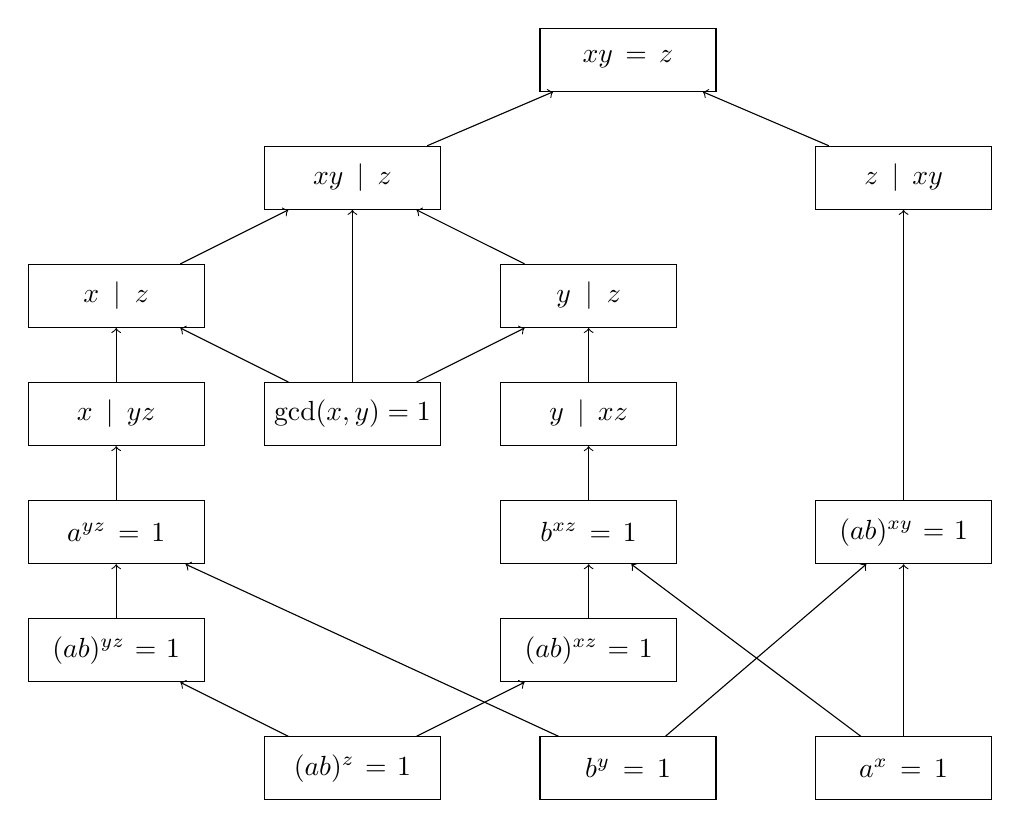
\begin{tikzpicture}[every node/.style={rectangle, draw, text width=2cm,text centered,minimum height=0.8cm}]
  \node (ass_x) at (12, 0) {$a^x=1$};
  \node (ass_y) at (8.5, 0) {$b^y=1$};
  \node (ass_z) at (5, 0) {$(ab)^z=1$};
  \node (abyz)  at (2, 1.5) {$(ab)^{yz}=1$};
  \node (abxz)  at (8, 1.5) {$(ab)^{xz}=1$};
  \node (ayz)   at (2, 3) {$a^{yz}=1$};
  \node (bxz)   at (8, 3) {$b^{xz}=1$};
  \node (abxy)  at (12, 3) {$(ab)^{xy}=1$};
  \node (xyz)   at (2, 4.5) {$x \mid yz$};
  \node (yxz)   at (8, 4.5) {$y \mid xz$};
  \node (ass_g) at (5, 4.5) {$\gcd(x,y)=1$};
  \node (xz)    at (2, 6) {$x \mid z$};
  \node (yz)    at (8, 6) {$y \mid z$};
  \node (xyz_)  at (5, 7.5) {$xy \mid z$};
  \node (zxy)   at (12, 7.5) {$z \mid xy$};
  \node (goal)  at (8.5, 9) {$xy = z$};

  \draw[->] (ass_x) -- (abxy);
  \draw[->] (ass_x) -- (bxz);
  \draw[->] (ass_y) -- (abxy);
  \draw[->] (ass_y) -- (ayz);
  \draw[->] (ass_z) -- (abyz);
  \draw[->] (ass_z) -- (abxz);
  \draw[->] (abyz) -- (ayz);
  \draw[->] (abxz) -- (bxz);
  \draw[->] (ayz) -- (xyz);
  \draw[->] (bxz) -- (yxz);
  \draw[->] (abxy) -- (zxy);
  \draw[->] (xyz) -- (xz);
  \draw[->] (yxz) -- (yz);
  \draw[->] (ass_g) -- (xz);
  \draw[->] (ass_g) -- (yz);
  \draw[->] (xz) -- (xyz_);
  \draw[->] (yz) -- (xyz_);
  \draw[->] (ass_g) -- (xyz_);
  \draw[->] (xyz_) -- (goal);
  \draw[->] (zxy) -- (goal);
\end{tikzpicture}
\caption{証明の流れ}
\label{fig:element_order}
\end{center}
\end{figure}
\end{prProof}

\subsubsection{\rProp{primitive_root_exists}の証明}
\begin{Theo}{\IND{剰余の定理}{しようよのていり}, polynomial remainder theorem}{polynomial_remainder_theorem}
多項式$f(x)$を$(x-a)$で割った余りは$f(a)$である。
同じことだが、ある多項式$g(x)$が存在し、
\begin{align*}
f(x) = (x-a)g(x) + f(a)
\end{align*}
を満たす。
\end{Theo}

\begin{Prop}{}{polynomial_root_n}
$p$を素数とする。
$\mathbb{Z}_p^*$を係数とする$n$次合同式の根は高々$n$個である。
\end{Prop}

\begin{prProof}{polynomial_root_n}
$f(n)$を$n$次合同式とする。
$f(x_0)=0$となる$x_0$が存在したとすると、\rTheo{polynomial_remainder_theorem}より
\begin{align*}
f(x) = (x-x_0)g(x) + f(x_0) = (x-x_0)g(x)
\end{align*}
もし、$x_0$以外の根$x_1$が存在すれば
\begin{align*}
0 = f(x_1) = (x_1-x_0)g(x_1)
\end{align*}
となるが、$x_1-x_0$は$p$で割り切れないから、$g(x_1)=0$。
つまり、$x_1$は$g(x)$の根でなければならない。

以上を念頭に置いて数学的帰納法を使う。

$n=1$のとき、$ax+b\equiv0\pmod{p}$はただ1つの根を持つ。
これは、\rProp{inverse_element_not_exists}からも分かる。

$n=k$のとき、$k-1$次合同式$g(x)$の根は高々$k-1$個であると仮定する。
$f(x)$の根は$x_0$以外は$g(x)$の根しかないので、$f(x)$の根は高々$k$個である。

よって題意は示された。
\end{prProof}

\begin{Lemm}{}{totient_function_multiplicative}
Eulerの$\varphi$関数は乗法的である。つまり、互いに素な$m,n$について、
\begin{align*}
\varphi(mn) = \varphi(m)\varphi(n)
\end{align*}
である。
\end{Lemm}

\begin{Lemm}{}{totient_function_even}
$n>2$のときEulerの$\varphi$関数$\varphi(n)$は偶数である。
\end{Lemm}

\begin{lmProof}{totient_function_even}
Eulerの$\varphi$関数が乗法的であることに注意する(\rLemm{totient_function_multiplicative})。
素数$p$に対して
\begin{align*}
\varphi(p^k) = p^{k-1}(p-1)
\end{align*}
であるから、$n$の素因数に奇素数があれば$(p-1)$が偶数になるので$\varphi(n)$は偶数になる。
また、$n$の因数に$2^k$(ここで$k>1$)があれば、$p^{k-1}$が偶数になるので$\varphi(n)$は偶数になる。
\end{lmProof}

\begin{Prop}{}{primitive_root_search_2p}
奇素数$p$、正整数$k$とし、$p^k$を法とする原始根を$g$とする。
$g$と$g+p^k$のうち、奇数である方が$2p^k$を法とする原始根である。
\end{Prop}

\begin{prProof}{primitive_root_exists}
2以上の自然数を次のように分割し、それぞれに原始根が存在する、あるいは存在しないことを示す。
\begin{enumerate}
 \item 2,4
 \item $2^k$。ただし、$k>2$
 \item 奇素数$p$
 \item $p^k$。ただし、$p$は奇素数で、$k>1$
 \item $2p^k$。ただし、$p$は奇素数で、$k\ge1$
 \item $mk$。ただし、$m$と$k$は互いに素で、$m>2, k>2$
\end{enumerate}

\noindent\textbf{2,4の場合}

$n=2,4$のとき、$g=1,3$がそれぞれの原始根である。

\noindent\textbf{$2^k$の場合}

どんな$a\in\mathbb{Z}_{2^k}^*$の位数も$\varphi(2^k)=2^{k-1}$未満であることを示す。
より具体的には、$a^{2^{k-2}}\equiv1\pmod{2^k}$を示せば、$a$の位数は高々$2^{k-2}$であり、$2^{k-1}$未満であることが分かって、原始根は存在しない。
$a$は奇数だから$a=2t+1$と書き直し、数学的帰納法を用いよう。

$k=3$のとき、
\begin{align*}
(2t + 1)^2 = 4t^2 + 4t + 1 = 4t(t+1) + 1 = 8T + 1 \equiv 1 \pmod{2^3}
\end{align*}
となり成立($t, t+1$のどちらかは偶数だから$4t(t+1)$は8で割り切れる)。

$k=m$のとき、$(2t+1)^{2^{m-3}}=2^{m-1}T+1$を仮定すると、
\begin{align*}
(2t + 1)^{2^{m-2}} = (2^{m-1}T+1)^2 = 2^{2(m-1)}T^2 + 2^mT + 1 = 2^m(2^{m-2}T^2 + T) + 1 \equiv 1 \pmod{2^m}
\end{align*}
となり、$a^{2^{k-2}}\equiv1\pmod{2^k}$が示された。
よって、原始根は存在しない。

\noindent\textbf{奇素数$p$の場合}

素数$p$に対して$p-1=\prod_{i=1}^kq_i^{e_i}$と素因数分解できるとする。
\rProp{polynomial_root_n}より、$(p-1)/q_i$次方程式
\begin{align*}
x^{(p-1)/q_i} \equiv 1 \pmod{p}
\end{align*}
を満たさない$X_i\in\mathbb{Z}_p^*$が存在する。
$Y_i=X_i^{(p-1)/q_i^{e_i}}$と置くと、
\begin{align*}
Y_i^{q_i^{e_i}} &\equiv X^{p-1} \equiv 1 \pmod{p}\\
Y_i^{q_i^{e_i-1}} &\equiv X^{(p-1)/q_i} \not\equiv 1 \pmod{p}
\end{align*}
を得る。
上式はFermatの小定理(\rTheo{Fermats-little-theorem})から得られるし、下式は$X$の前提条件を思い返せば当然の結論だ。
このことから$\mbox{ord}(Y_i)=q_i^{e_i}$を得るが、これはすべての$p-1$の素因数に言える。
そこで、\rProp{element_order}の3を適用すると、
\begin{align*}
\mbox{ord}(Y_1Y_2\cdots Y_k) = q_1^{e_1}q_2^{e_2} \cdots q_k^{e_k} = p-1
\end{align*}
を得る。
よって、$\prod_{i=1}^k Y_i$は$p$を法とする原始根である。

\noindent\textbf{$p^k$の場合}

\rProp{primitive_root_search}より原始根が存在する。

\noindent\textbf{$2p^k$の場合}

\rProp{primitive_root_search_2p}より原始根が存在する。

\noindent\textbf{$mk$の場合}

$mk$(ただし、$m$と$k$は互いに素で、$m>2, k>2$)のとき、\rLemm{totient_function_even}より$\varphi(m),\varphi(k),\varphi(mk)$は偶数であるから、それぞれを2で割っても問題ない。
最終的に、任意の$a\in\mathbb{Z}_n^*$に対して
\begin{align*}
a^{\frac{\varphi(mk)}{2}} \equiv 1 \pmod{mk}
\end{align*}
を示す。
これによって、$a$の位数は$\varphi(mk)$未満であることが分かり、原始根は存在しないと結論付けられる。
それには、$\bmod{m},\bmod{k}$それぞれにおける$a^{\varphi(mk)/2}$を評価してみる。
\rLemm{totient_function_multiplicative}より、$\varphi(mk)=\varphi(m)\varphi(k)$であることを思い出すと、
\begin{align*}
a^{\frac{\varphi(mk)}{2}} &= (a^{\varphi(m)})^{\frac{\varphi(k)}{2}} \equiv 1 \pmod{m}\\
a^{\frac{\varphi(mk)}{2}} &= (a^{\varphi(k)})^{\frac{\varphi(m)}{2}} \equiv 1 \pmod{k}
\end{align*}
となって、$a^{\varphi(mk)/2}\equiv1\pmod{m}$および$a^{\varphi(mk)/2}\equiv1\pmod{k}$を得る。
この2式から、\rTheo{chinese_remainder_theorem}より$a^{\varphi(mk)/2} \equiv 1 \pmod{mk}$が得られる。
\end{prProof}
